% IEEE standard conference template; to be used with:
%   spconf.sty  - LaTeX style file, and
%   IEEEbib.bst - IEEE bibliography style file.
% --------------------------------------------------------------------------

\documentclass[letterpaper]{article}
\usepackage{spconf,amsmath,amssymb,graphicx}
\graphicspath{{./plots/}}
\usepackage[linesnumbered,ruled]{algorithm2e}

% Example definitions.
% --------------------
% nice symbols for real and complex numbers
\newcommand{\R}[0]{\mathbb{R}}
\newcommand{\C}[0]{\mathbb{C}}
\newcommand{\argmax}[1]{\underset{#1}{\operatorname{arg}\,\operatorname{max}}\;}

% bold paragraph titles
\newcommand{\mypar}[1]{{\bf #1.}}

% Title.
% ------
\title{Fast Gaussian Process Upper Confidence Bound (GP-UCB) implementation}
%
% Single address.
% ---------------
\name{Daan Nilis, Linus Handschin, Julien Lamour} 
\address{Department of Computer Science\\ ETH Z\"urich\\Z\"urich, Switzerland}

% For example:
% ------------
%\address{School\\
%		 Department\\
%		 Address}
%
% Two addresses (uncomment and modify for two-address case).
% ----------------------------------------------------------
%\twoauthors
%  {A. Author-one, B. Author-two\sthanks{Thanks to XYZ agency for funding.}}
%		 {School A-B\\
%		 Department A-B\\
%		 Address A-B}
%  {C. Author-three, D. Author-four\sthanks{The fourth author performed the work
%		 while at ...}}
%		 {School C-D\\
%		 Department C-D\\
%		 Address C-D}
%

\begin{document}
%\ninept
%
\maketitle
%

\begin{abstract}
Describe in concise words what you do, why you do it (not necessarily
in this order), and the main result.  The abstract has to be
self-contained and readable for a person in the general area. You
should write the abstract last.
\end{abstract}

\section{Introduction}\label{sec:intro}

In this section, we motivate our work and describe the references we used as starting points.

\mypar{Motivation} Many applications require the extraction of the maximum of an unknown function, usually expensive to sample. Advertiser systems, that are aiming to maximize the click-through rate, is such an example. In a more basic scenario, one could try to find the location of the highest temperature in a building by sequentially activating as few sensors as possible in the building.

Performance matters here for several reasons. In many application, the time span between the moment the sampling result is known and the moment the decision which point to sample next has to be sampled is to be minimized. Moreover, the search space might be very large, making that first constraint harder to fulfill. The example of the advertiser system is a good illustration of these two reasons, where one desires very short delay between the sampling of the function (a specific add was displayed to a user, we observe whether he clicked it or not), and deciding the next point to sample (which add to display to the next user) and can have a very extensive search space (many adds and users to choose from).

Even if the GP-UCB algorithm repetedly performs several similar steps in each iteration, it is still inherently sequential, since the result of one iteration has to be known in order to proceed to the next one. Fast implementations require thinking on the way code has to be vectorized since part of the working set is growing at each iteration.

We are presenting here a vectorized implementation of the GP-UCB algorithm for the 2D scenario (function and search grid in $\mathbb{R}$) with a fixed kernel.

\mypar{Related work} The implementation was based on \cite{Krause:09} which describes the GP-UCB algorithm in more details and provides its pseudocode, and \cite{rasmussen2006gaussian} which provides the pseudocode to perform a Bayesian update.

\section{Background: the GP-UCB algorithm}\label{sec:background}

In this section, we define the GP-UCB algorithm and perform a cost analysis. \textbf{TODO: add explanation of Upper Confidence Bound: Linus}.

\mypar{Radial Basis Function (RBF) kernel}
The RBF kernel on two samples $\mathbf{x}$ and $\mathbf{x'}$, represented as feature vectors in some input space, is defined as:
\begin{equation*}
    K(\mathbf{x}, \mathbf{x'}) = \exp\left(-\frac{\lVert \mathbf{x} - \mathbf{x'} \rVert}{2\sigma^2}\right)
\end{equation*}

\mypar{GP-UCB algorithm}
We fixed the kernel $k$ to be the RBF kernel in our implementation in order to perform optimization on its computation as well as for having a stricly defined cost measure to deduce performance. The $\beta$ parameter is chosen by the user and expresses the trade off between exploration (points where uncertainty is high are sampled) and exploitation (points where the function is known to be relatively high are sampled) that the user desires to make. The Bayesian update mentioned in Algorithm~\ref{alg:gpucb} is detailed in Algorithm~\ref{alg:bayesianupdate}.
\begin{algorithm}
    \label{alg:gpucb}
    \SetKwInOut{Input}{Input}
    \SetKwInOut{Output}{Output}    
    \Input{Input space $D$; GP Prior $\mu_0 = 0$, $\sigma_0$, $k$, $\beta$}
    \Output{$\mu_t$ and $\sigma_t$, the estimations for the mean and variance at each iteration.}
    \For{$t=1,2,...$}
        {
            Choose $\mathbf{x_t} = \argmax{\mathbf{x}\in D} \mu_{t-1}(\mathbf{x}) + \sqrt{\beta_t}\sigma_{t-1}(\mathbf{x})$\\
            Sample $y_t=f(\mathbf{x_t}) + \epsilon_t$\\
            Perform Bayesian update to obtain $\mu_t$ and $\sigma_t$
        }
    \caption{The GP-UCB algorithm. \cite{Krause:09}}
\end{algorithm}

\mypar{Gaussian Process} The function $f$ that we aim to estimate is modeled as a Gaussian Process (GP), which is a collection of dependent random variables, one for each $\mathbf{x} \in D$. A $GP(\mu(\mathbf{x}), k(\mathbf{x}, \mathbf{x'}))$ is specified by its mean function $\mu(\mathbf{x})=\mathbb{E}[f(\mathbf{x})]$ and covariance (or kernel) function $k(\mathbf{x}, \mathbf{x'})= \mathbb{E}[(f(x)-\mu(\mathbf{x}))(f(x')-\mu(\mathbf{x'}))]$. For GP not conditioned on data (as it is the case here), we assume $\mu \equiv 0$. Moreover, $k(\mathbf{x}, \mathbf{x}), \mathbf{x} \in D$ is restricted to be less or equal to 1, which is fulfilled by the RBF kernel.
\begin{algorithm}
    \label{alg:bayesianupdate}
    \SetKwInOut{Input}{Input}
    \SetKwInOut{Output}{Output}    
    \Input{$X$ (inputs), $\mathbf{y}$ (targets), $k$ (covariance function), $\sigma_n^2$ (noise level), $\mathbf{x_*}$ (test input)}
    \Output{$\bar{f_*}$ (mean), $\mathbb{V}[f_*]$ (variance)}
    $L := \textnormal{cholesky}(K+\sigma^2_nI)$\\
    $\mathbf{\alpha}:=L^T\backslash(L\backslash\mathbf{y})$\\
    $\bar{f_*}:=\mathbf{k_*}^T\mathbf{\alpha}$\\
    $\mathbf{v}:=L\backslash\mathbf{k_*}$\\
    $\mathbb{V}[f_*]:=k(\mathbf{x_*}, \mathbf{x_*})-\mathbf{v}^T\mathbf{v}$\\
    \Return {$\bar{f_*}, \mathbb{V}[f_*]$}
    \caption{Predictions for Gaussian process regression. \cite{rasmussen2006gaussian}}
\end{algorithm}


\mypar{Cost Analysis}
Based on our experiments, we decided to use single precision floating point numbers since it was sufficient to retrieve the maximum point of the function with the RBF kernel and allowed higher performance.
The cost measure is defined in the following way:
\begin{align*}
    &C(N,\mathcal{I})\\
    &=C_{add}(N,\mathcal{I}) + C_{mul}(N,\mathcal{I}) + C_{div}(N,\mathcal{I})+C_{exp}(N,\mathcal{I})\\
    &=n_{add}(N,\mathcal{I}) + n_{mul}(N,\mathcal{I}) + n_{div}(N,\mathcal{I}) + 20n_{exp}(N,\mathcal{I})
\end{align*}
where:
\begin{itemize}
    \item The search grid contains $N^2$ points.
    \item $\mathcal{I}$ is the number of iterations performed.
    \item $n_{flop}(N,\mathcal{I})$ is the number of time the specific single precision $flop$ is executed for given $N$ and $\mathcal{I}$.
    \item The divisions and exponentials come from the RBF kernel, and the cost would change with the use of another kernel.
\end{itemize}

We instrumented the code in order to have the exact flops count, but the asymptotic measure is the following:
\begin{equation*}
    W(N, \mathcal{I}) = N^2*\left(\sum_{i=1}^\mathcal{I}(i^2 + i) + \mathcal{I} * k\right) + O(\mathcal{I}^3)
\end{equation*}

\textbf{TODO: High-level explanation of where the numbers come from.}

Also state what is
known about the complexity (asymptotic usually) 
about your problem (including citations).

Don't talk about "the complexity of the algorithm.'' It's incorrect,
remember (Lecture 2)?


\section{Your Proposed Method}\label{sec:yourmethod}

In this section, we ...

We assumed $N$ to be divisible by 8. The reason for that is that 8 floating point numbers fit in a AVX vector and this assumption therefore simplifies the vectorization.

\mypar{Baseline} We implemented the baseline ourselves, using C code without trying to do any optimization at first, as if we wouldn't have taken the class. The high-level overview of the baseline (valid for the optimized version as well) is the following:
\begin{enumerate}
    \item \texttt{run} performs a learning step for each iteration: \texttt{for i in 1..$\mathcal{I}$: learn}.
    \item \texttt{learn} samples the argmax point (line 2 of Algorithm~\ref{alg:gpucb}) depending on the current values of $\mu$, the uncertainty $\sigma$ and the chosen $\beta$ value and calls \texttt{gp regression} after each sampling.
    \item \texttt{gp regression} performs a Bayesian update (as described in Algorithm~\ref{alg:bayesianupdate}) for each point in the search grid in order to obtain the updated $\mu$ and $\sigma$ with the additional information brought the latest sampled point.
    \item Several minor helper functions were declared to improve readability. \texttt{incremental cholesky} and \texttt{cholesky solve} are examples of these.
\end{enumerate}

\mypar{Operational intensity} The number of operations $W(N, \mathcal{I})$ was detailed in the previous operation. Since the only element that has to be loaded is the search grid, containing $2 * 4 * N^2$ points in the 2D scenario, the operational intensity is the following:
\begin{align*}
    I(N, \mathcal{I}) &= \frac{W(N, \mathcal{I})}{Q(N, \mathcal{I})} \\
    &= \frac{N^2*\sum_{i=1}^\mathcal{I}(i^2+i)+O(N^2\mathcal{I}+\mathcal{I}^3)}{8*N^2}\\
    &= \frac{2\mathcal{I}^3}{3}+O\left(\frac{\mathcal{I}^3}{N^2}+\mathcal{I}\right) >> 1
\end{align*}

As explained earlier in the Cost Analysis paragraph, the bottleneck is triangle solve... explain more

\mypar{Incremental Cholesky} Daan

\mypar{Triangle solve} Daan

\mypar{8x8 matrix-matrix multiplication (MMM)} As explained in the previous paragraph, we require high-performance 8x8 MMM since it is part of the bottleneck routine. We implemented it in a vectorized fashion using fused multiply-add (FMA). The performance reached is discussed in Section~\ref{sec:exp}.

\mypar{Fuse Bayesian update and argmax} In a naive implementation, one would first perform the Bayesian update for all points on the grid in order to obtain the new values of $\mu$ and $\sigma$, and then go through every entry a second time in order to identify the maximum value of $\mu(\mathbf{x})+\sqrt{\beta}\sigma(\mathbf{x})$. This argmax step can actually be done during the update itself by memorizing the highest value, saving an entire pass through $\mu$ and $\sigma$.

\section{Experimental Results}\label{sec:exp}

Here you evaluate your work using experiments. You start again with a
very short summary of the section. The typical structure follows.

\mypar{Experimental setup} For the following measurements, we have been using the machines available in the CAB computer labs, namely: Intel core i7 (Skylake) @3.4GHz, L1: 32 KB, L2: 256 KB, L3: 8 MB. GCC 4.8.5 was used for compilation with the flags -O3 and -fno-tree-vectorize.

Then explain what input you used and what range of sizes. The idea is to give enough information so the experiments are reproducible by somebody else on his or her code.

\mypar{Results}
Next divide the experiments into classes, one paragraph for each. In the simplest case you have one plot that has the size on the x-axis and the performance on the y-axis. The plot will contain several lines, one for each relevant code version. Discuss the plot and extract the overall performance gain from baseline to best code. Also state the percentage of peak performance for the best code. Note that the peak may change depending on the situation. For example, if you only do additions it would be 12 Gflop/s
on one core with 3 Ghz and SSE and single precision floating point.

Do not put two performance lines into the same plot if the operations count changed significantly (that's apples and oranges). In that case first perform the optimizations that reduce op count and report the runtime gain in a plot. Then continue to optimize the best version and show performance plots.

\mypar{Incremental Cholesky} Daan

\mypar{Triangle solve} Daan

\mypar{8x8 matrix-matrix multiplication} Performance reached was xxx f/c.

{\bf You should}
\begin{itemize}
\item Follow the guide to benchmarking presented in class, in particular
\item very readable, attractive plots (do 1 column, not 2 column plots
for this class), proper readable font size. An example is below (of course you can have a different style),
\item every plot answers a question, which you pose and extract the
answer from the plot in its discussion
\end{itemize}
Every plot should be discussed (what does it show, which statements do
you extract).

\section{Conclusions}

Here you need to briefly summarize what you did and why this is
important. {\em Do not take the abstract} and put it in the past
tense. Remember, now the reader has (hopefully) read the paper, so it
is a very different situation from the abstract. Try to highlight
important results and say the things you really want to get across
(e.g., the results show that we are within 2x of the optimal performance ... 
Even though we only considered the DFT, our optimization
techniques should be also applicable ....) You can also formulate next
steps if you want. Be brief.

\section{Further comments}

Here we provide some further tips.

\mypar{Further general guidelines}

\begin{itemize}
\item For short papers, to save space, I use paragraph titles instead of
subsections, as shown in the introduction.

\item It is generally a good idea to break sections into such smaller
units for readability and since it helps you to (visually) structure the story.

\item The above section titles should be adapted to more precisely
reflect what you do.

\item Each section should be started with a very
short summary of what the reader can expect in this section. Nothing
more awkward as when the story starts and one does not know what the
direction is or the goal.

\item Make sure you define every acronym you use, no matter how
convinced you are the reader knows it.

\item Always spell-check before you submit (to me in this case).

\item Be picky. When writing a paper you should always strive for very
high quality. Many people may read it and the quality makes a big difference.
In this class, the quality is part of the grade.

\item Conversion to pdf (latex users only): 

dvips -o conference.ps -t letter -Ppdf -G0 conference.dvi

and then

ps2pdf conference.ps
\end{itemize}

\mypar{Graphics} For plots that are not images {\em never} generate (even as intermediate step)
jpeg, gif, bmp, tif. Use eps, which means encapsulate postscript, os pdf. This way it is
scalable since it is a vector graphic description of your graph. E.g.,
from Matlab, you can export to eps or pdf.

Here is an example of how to get a plot into latex
(Fig.~\ref{fftperf}). Note that the text should not be any smaller than shown.

\begin{figure}\centering
  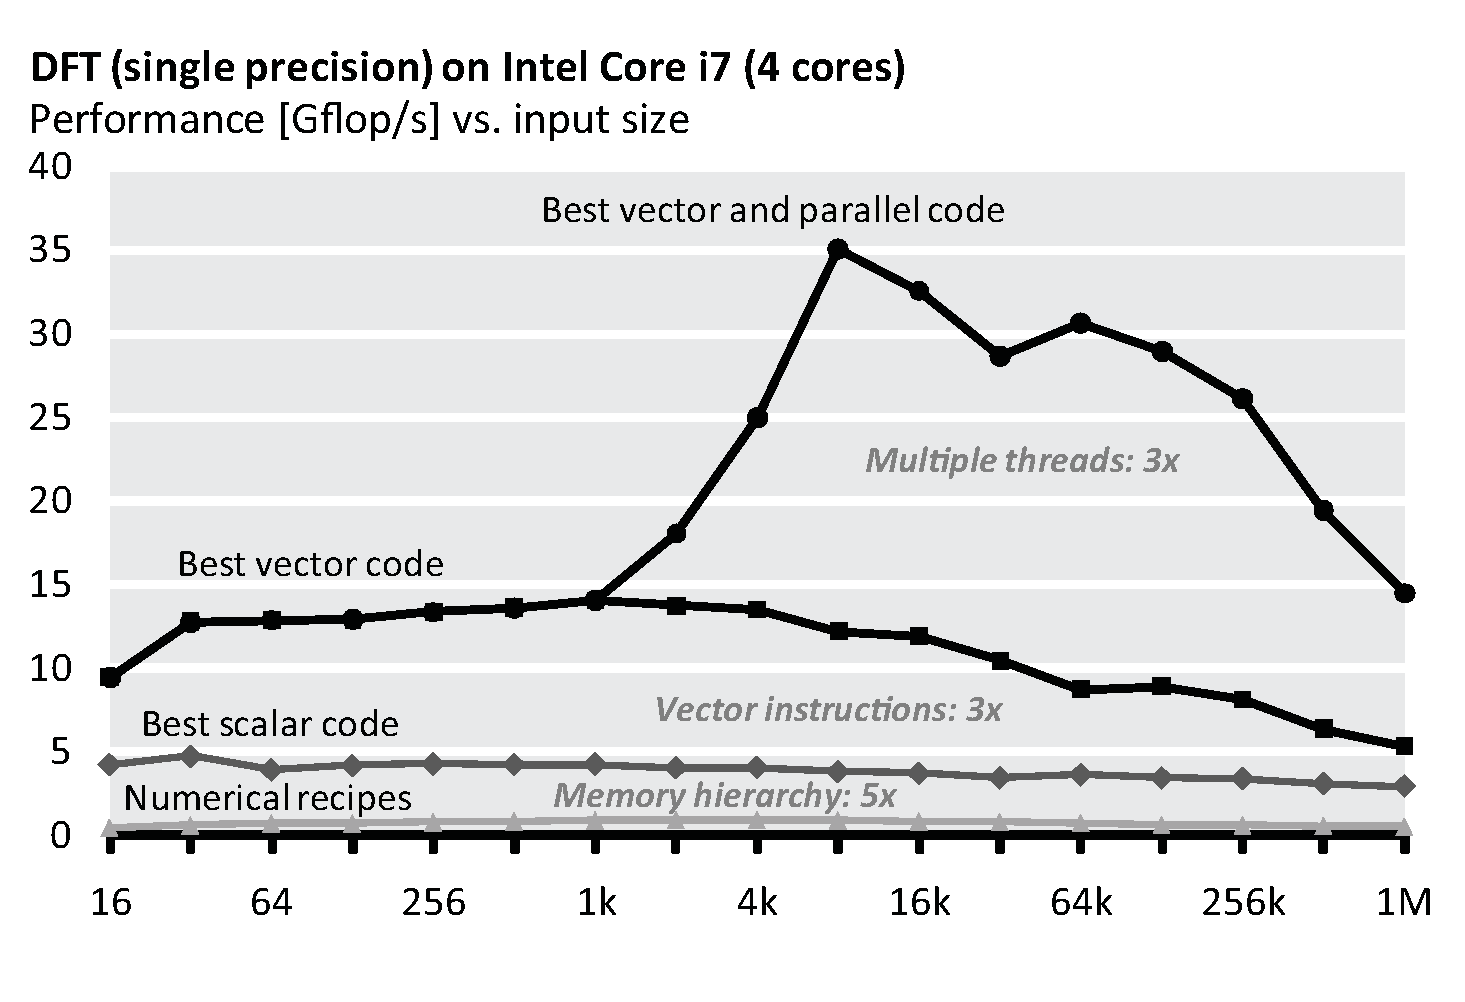
\includegraphics[scale=0.33]{dft-performance.eps}
  \caption{Performance of four single precision implementations of the
  discrete Fourier transform. The operations count is roughly the
  same. {\em The labels in this plot are too small.}\label{fftperf}}
\end{figure}



% References should be produced using the bibtex program from suitable
% BiBTeX files (here: bibl_conf). The IEEEbib.bst bibliography
% style file from IEEE produces unsorted bibliography list.
% -------------------------------------------------------------------------
\bibliographystyle{IEEEbib}
\bibliography{bibl_conf}

\end{document}

